\documentclass[a4paper,11pt]{letter}
\usepackage{fontspec}
\setromanfont[
BoldFont=cambriab.ttf,
ItalicFont=cambriai.ttf,
BoldItalicFont=cambriabi.ttf,
]{cambria.ttf}
\usepackage{hyperref}
\usepackage[left=0.7in, right=0.7in, bottom=0.7in, top=1in]{geometry}
\usepackage{wrapfig}
\usepackage[official]{eurosym}
\usepackage{graphicx}
\graphicspath{ {images/}}

\begin{document}
\noindent  \large{\textbf{Ivan Viola -- Curriculum Vitae~~~~~~~~~~~~~~~~~~~~~~~~~~~~~~~~~~~~~~~~~~~~~~~~~~~~~~~~~~~~~~~~~~~~~~\href{https://orcid.org/0000-0003-4248-6574/}{ORCID: 0000-0003-4248-6574}}} \\
\vspace{-2ex} 
\hrule 
\normalsize

\begin{wrapfigure}{r}{0.2\linewidth}
\centering
\setlength{\fboxsep}{0pt}%
\setlength{\fboxrule}{1pt}%
\fbox{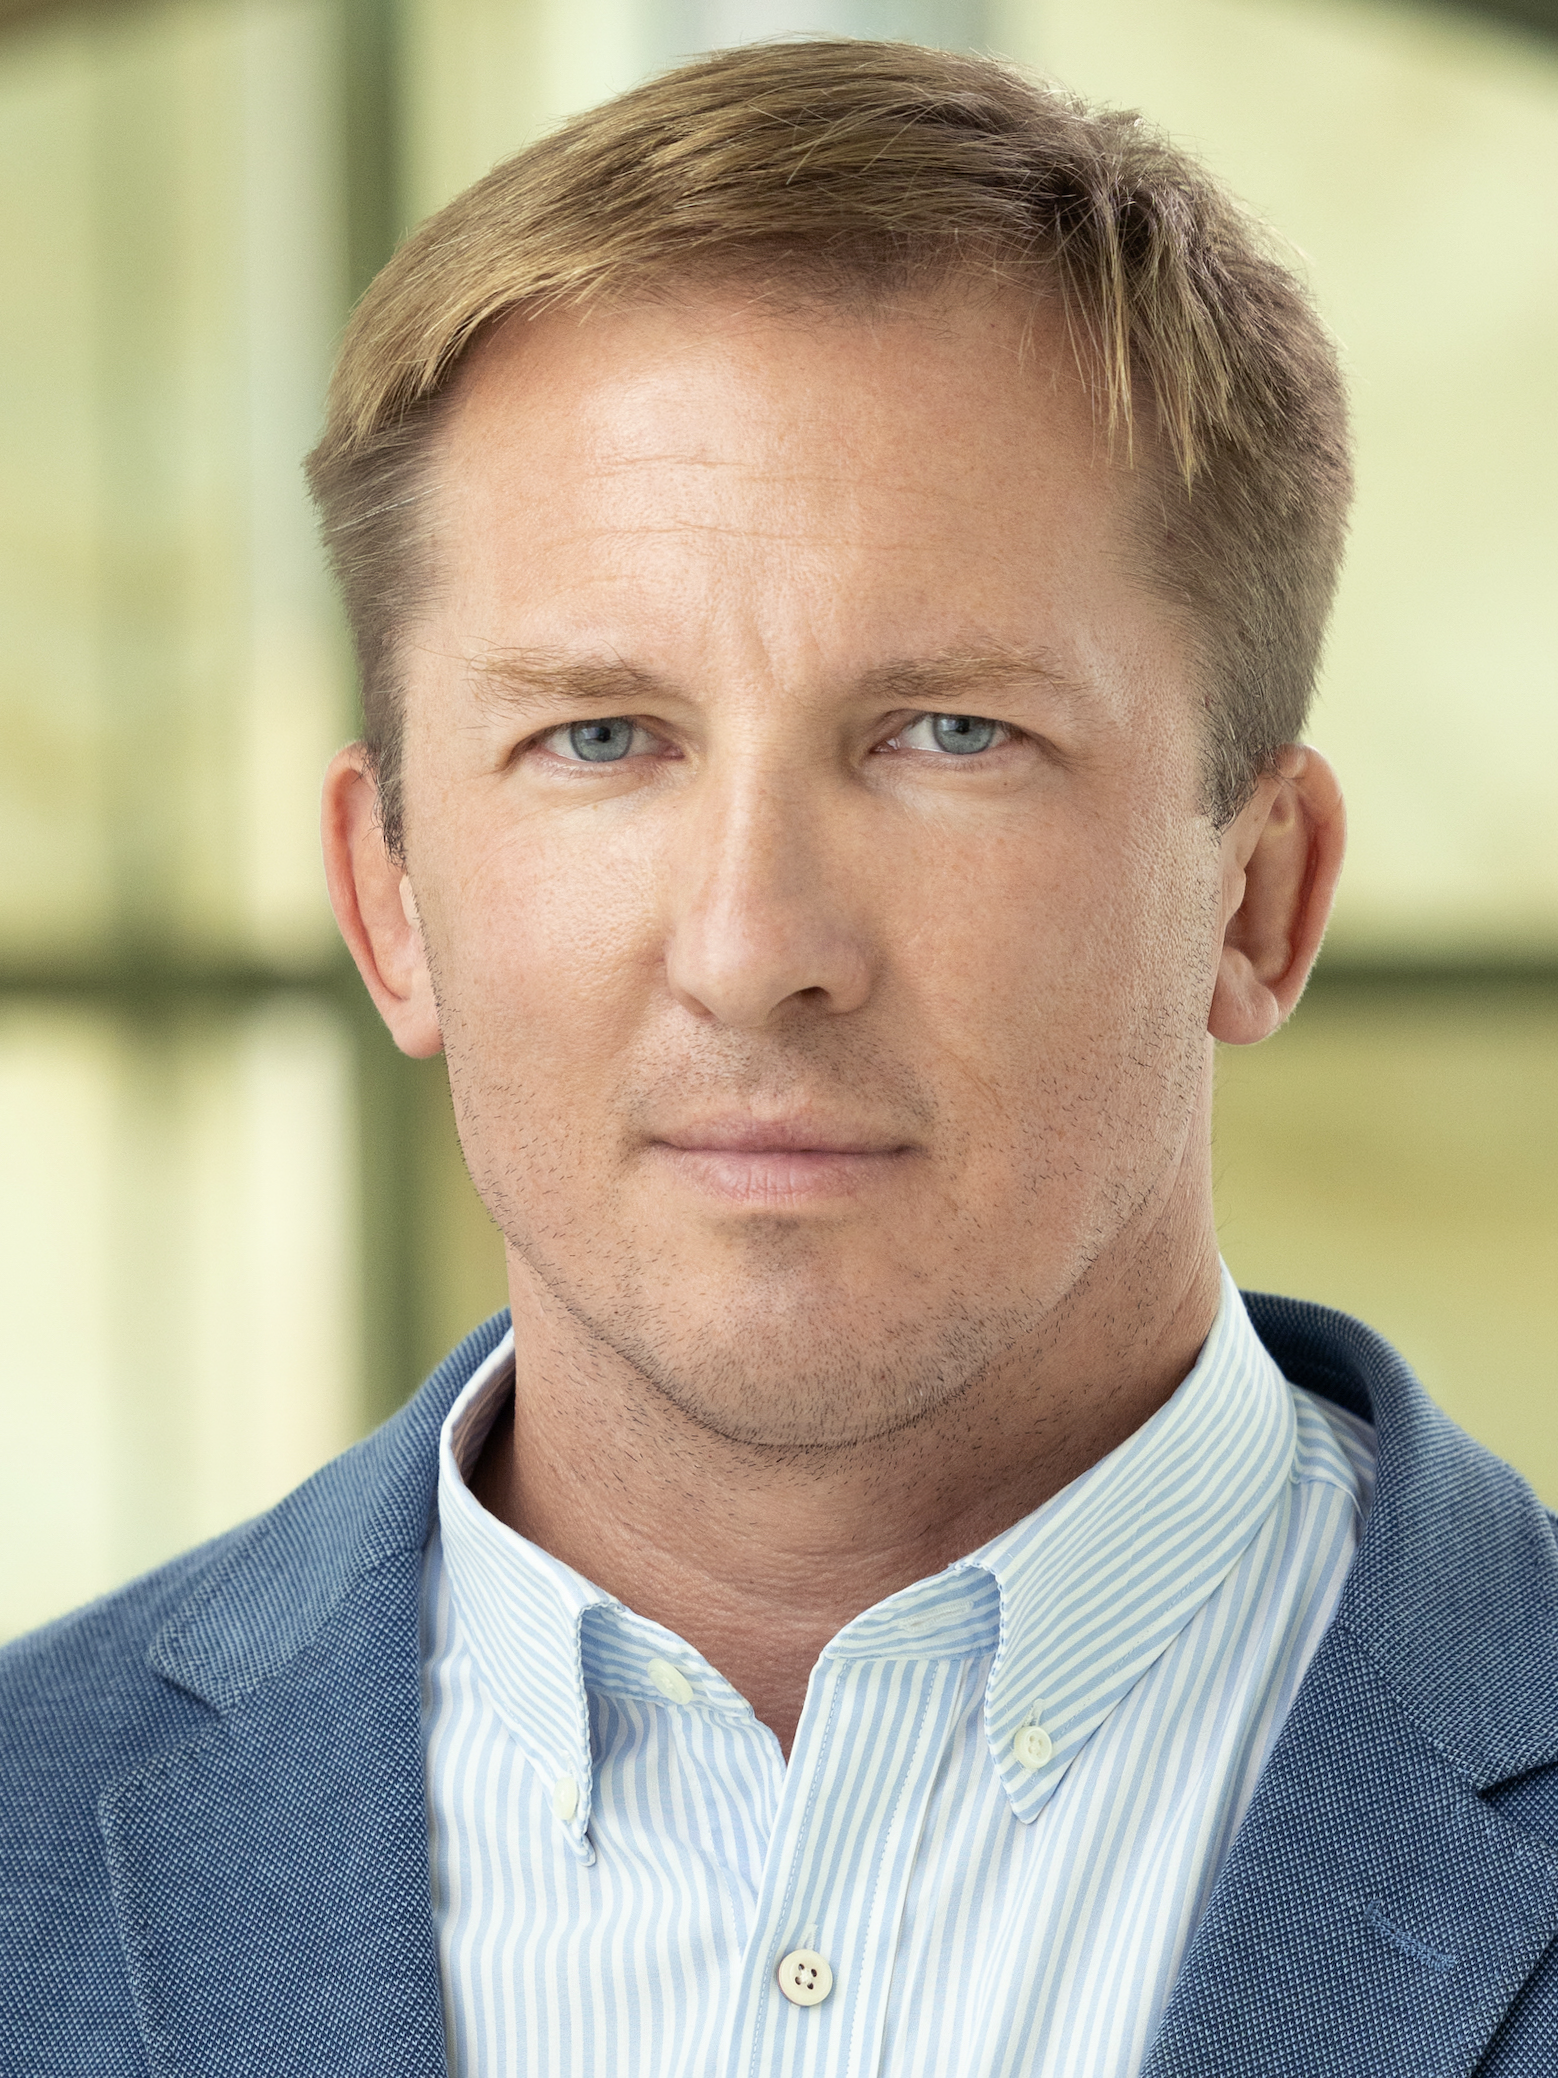
\includegraphics[width=3.1cm]{images/Ivan Viola-3-4.png}}%
\end{wrapfigure}
~\\
King Abdullah University of Science and Technology (KAUST) \\
Computer, Electrical and Mathematical Science and Engineering \\ 
Computer Science \\
Thuwal 23955, Saudi Arabia \\
\href{mailto:ivan.viola@kaust.edu.sa}{ivan.viola@kaust.edu.sa} \\
+966 12 8080617\\
~

%\textbf{Personal Information:}\\
%     Born: 25.06.1977, Bratislava, Czechoslovakia \\
%     Nationality: Slovak \\
%     Status: married (Sonia Viola), two children (Emma Viola \& Ella Viola)\\

~\\

\textbf{Research Interests:} visualization, computer graphics\\

\textbf{Positions:} \\
\setlength{\tabcolsep}{0.5em}
\begin{tabular}{l|l}
%\hline
    2018 -- & \textbf{KAUST}, Saudi Arabia, \href{http://nanovis.kaust.edu.sa/}{nanovis.kaust.edu.sa}  \\
2022 -- 2023     & Program Chair\\
2021 --     & Professor\\
     & Associate Professor\\
\hline
    2017 -- & \textbf{Nanographics GmbH}, Austria, \href{http://www.nanographics.at/}{nanographics.at}  \\
     2018 -- & Co-founder\\
     & CEO \\
\hline
    2013 -- 2018 & \textbf{TU Wien}, Austria, \href{http://www.cg.tuwien.ac.ac.at/}{www.cg.tuwien.ac.at}  \\
     2017 -- & Associate Professor \\
     & Assistant Professor\\
\hline
    2006 -- 2015 & \textbf{University of Bergen}, Norway, \href{http://vis.uib.no/}{vis.uib.no} \\
     2013 -- & Adjunct Professor (20\%) \\
     2011 -- & Professor  \\
     2008 -- & Associate Professor \\
     & Postdoctoral Fellow \\
\hline
    2008 -- 2012 & \textbf{Christian Michelsen Research}, Norway, \href{http://www.cmr.no/}{www.cmr.no} \\
      & Scientific Advisor   (20\%)\\
\hline
    2002 -- 2006 & \textbf{TU Wien}, Austria, \href{http://www.cg.tuwien.ac.ac.at/}{www.cg.tuwien.ac.at}  \\
     2005 -- & Postdoctoral Research Associate, \href{http://www.cg.tuwien.ac.at/research/vis/exvisation/}{ExVisation project} \\
     & Research Assistant \href{http://www.cg.tuwien.ac.at/research/vis/adapt/}{ADAPT project} \\
\hline
\multicolumn{2}{l}{~}\\
\multicolumn{2}{l}{\hspace{-0.2cm}\textbf{Qualifications:}} \\
%\hline
Habilitation:     &  \textbf{Effective Visual Representations} \\
Title: & Privatdozent (\textbf{venia docendi}), \textbf{TU Wien}, Austria, Computer Science, 2016 \\
     &  \emph{compatible with Senior Lecturer}\\
\hline
Dissertation:      & \textbf{Importance-Driven Expressive Visualization} \\
Title: & Doctor technicae (\textbf{Dr. techn.}), \textbf{TU Wien}, Austria, Computer Science, 2005 \\
Supervisor:  & M. Eduard Gröller \\
     & \emph{compatible with Doctor of Philosophy (PhD)}\\
\hline
Master Thesis: & \textbf{Applications of Hardware-Accelerated Filtering in Computer Graphics} \\
Title: & Diplom-Ingenieur (\textbf{Dipl.-Ing.}), \textbf{TU Wien}, Austria, Computer Science, 2002 \\
Supervisors:      & Markus Hadwiger, Helwig Hauser, M. Eduard Gröller \\
     & \emph{compatible with Master of Science (MSc)}\\
\end{tabular}

\small
\begin{tabular}{l| l}
\multicolumn{2}{l}{\large{\textbf{Externally Funded Projects:}}} \\
%\hline
%\textbf{Ongoing:} & \\
%\end{tabular}
%\\
%\begin{tabular}{l| l}
%\textbf{Completed:} & \\
2022 -- 2024 & \textbf{Commercial Development and Validation of MesoCraft Software} \\
 & \textbf{for 3D Modelling and Animation of Cryo-Electron Tomography Data} (\#1068) \\
Role: & Proposer, PI \\
Agency: & KAUST Research Translation Fund \\
Scope: & web-based molecular modeling system\\
Volume: & 883 000 \$ \\
\hline
2021 -- 2023 & \textbf{MesoNet: Rapid 3D Modeling and Visualization of Mesocale Biological Structures} (\#757) \\
Role: & Proposer, PI, Supervisor \\
Agency: & KAUST Competitive Research Grants Program \\
Scope: & basic research in microscopy visualization \\
Volume: & 399 825 \$ \\
\hline
2021 -- 2022 & \textbf{AI-Powered 3D Volume Visualization of Cryo-EM Tomography} (\#908) \\
Role: & Proposer, PI \\
Agency: & KAUST Impact Acceleration Fund \\
Scope: & web-based microscopy visualization system\\
Volume: & 100 000 \$ \\
\hline
2017 -- 2020 & \textbf{Integrative Visual Abstraction of Molecular Data} (\#I2953) \\
Role: & Proposer, PI, Supervisor \\
Agency: & FWF Austrian Science Fund: Joint Projects (with Inria, France) \\
Scope: & basic research in illustrative visualization \\
Volume: & 148 000 \euro{} \\
\hline
2017 -- 2019 & \textbf{BioNetIllustration: User centric illustrations of biological networks} (\#747985) \\
Role: & Co-Proposer, Supervisor \\
Agency: & European Commission: Marie Curie Fellowship (ranked as \#38 out of 800+) \\
Scope: & basic research in illustrative graph visualization \\
Volume: & 166 000 \euro{} \\
\hline
2013 -- 2020 & \textbf{Visual Computing: Illustrative Visualization} (\#VRG11-010) \\
Role: & Proposer, PI, Supervisor \\
Agency: & WWTF Vienna Science and Technology Fund: Vienna Research Groups 2011\\
Scope: & basic research in visualization of biological structures \\
Volume: & 1 500 000 \euro{} \\
\hline
2013 -- 2017 & \textbf{Illustrative Visualization of Processes} (\#PCIG13-GA-2013-618680) \\
Role: & Proposer, Fellow \\
Agency: & European Commission: Marie Curie Career Integration Grant (ranked as \#5 out of 144) \\
Scope: & grant for supporting fellow during the relocation period \\
Volume: & 100 000 \euro{} \\
\hline
2012 -- 2015 & \textbf{PhysioIllustration: Illustrative Visualization of Physiological Processes} (\#218023) \\
Role: & Proposer, PI, Researcher \\
Agency: & Norwegian Research Council: FRIPRO \\
Scope: & basic research in illustrative visualization of physiological processes \\
Volume: & 8 700 000 NOK \\
\hline
2009 -- 2012 & \textbf{IllustraSound: Supporting Communication with Illustrative Visualization} (\#193170) \\
Role: & Proposer, PI, Supervisor \\
Agency: & Norwegian Research Council: VERDIKT \\
Scope: & basic and applied research project on illustrative ultrasound visualization \\
Volume: & 8 300 000 NOK \\
\hline
2009 -- 2012 & \textbf{Geoillustrator: Illustrative Visualization of Geological Data and Models}  \\
Role: & Supervisor \\
Agency: & Statoil (Equinor) Academia Agreement \\
Scope: & basic research project on illustrative geological visualization \\
Volume: & 2 600 000 NOK \\
\hline
2005 -- 2008 & \textbf{ExVisation: Importance-Based Feature Enhancement in Volume Imaging} (\#P18322) \\
Role: & Proposer, Researcher \\
Agency: & FWF Austrian Science Fund: Research Projects \\
Scope: & basic research project on illustrative volume visualization \\
Volume: &  213 000 \euro{} \\
\hline
\end{tabular}

\newpage
\normalsize
\begin{tabular}{l| l}
\multicolumn{2}{l}{\large{\textbf{Recognition:}}} \\
\hline
\multicolumn{2}{l}{\textbf{~}} \\
\multicolumn{2}{l}{\textbf{Awards:}} \\
2023 & IEEE VIS Best Paper Honorable Mention\\
2020 & Computer Graphics Forum Cover Contest\\
2019 & 1st Place Graph Drawing Contest\\
2018 & IEEE VIS Best Paper Honorable Mention\\
2017 & IEEE VIS Best Paper Honorable Mention\\
2016 & Austrian Computer Graphics Award for the Best Technical Solution\\
2016 & Honorable Mention of EG VCBM\\
2015 & Best Paper Award, SCCG\\
2015 & Best Paper of EG VCBM\\
2013 & 1st Place Eurographics Dirk Bartz Prize for Visual Computing in Medicine\\
2013 & Second Best Paper Award of SCCG\\
2012 & Best Papers of SBIM\\
2012 & Second Best Paper Award of SCCG\\
2010 & Best Student Paper Award Graphics Interface\\
2009 & Honorable Mention for Best Paper at the EG UK TPCG\\
2004 & Best Paper Nomination IEEE Visualization\\
2004 & Second Best Paper Award of SCCG \\
\hline
\multicolumn{2}{l}{\textbf{~}} \\
\multicolumn{2}{l}{\textbf{Plenary Talks:}} \\
2023 & \emph{3D Modeling of Cellular Mesoscale} \\
 & EG Workshop on Molecular Graphics and Visual Analysis of Molecular Data, Leipzig, Germany \\
2019 & \emph{Automated Visualization: The Future of In Situ Processing?} \\
 & EG Symposium on Parallel Graphics and Visualization, Porto, Portugal \\
2018 & \emph{Large-Scale Interactive Visualization of Protein Environments} \\
 & Visualizing Biological Data - VizBi, Broad Institute of MIT and Harvard, USA \\
2017 & \emph{Visual Integration of Molecular and Cell Biology} \\
 & EG SIGRAD, Norrk\"oping, Sweden \\
2017 & \emph{Visual Integration of Molecular and Cell Biology} \\
 & CESCG Conference, Smolenice, Slovakia \\
2017 & \emph{Multi-Scale Molecular Data Visualization} \\
 & Computer Vision Winter Workshop, Retz, Austria \\ 
2013 & \emph{Declarative Visualization} \\
 & Spring Conference on Computer Graphics, Smolenice, Slovakia \\
2011 & \emph{Passing Through the Trough of Disillusionment of Illustrative Visualization} \\
 & EG-UK Theory and Practice in Computer Graphics, Warwick, UK \\
\hline
\end{tabular}

\begin{tabular}{l| l}
\multicolumn{2}{l}{\large{\textbf{Elected Service:}}} \\
\hline
\multicolumn{2}{l}{\textbf{~}} \\
\multicolumn{2}{l}{\textbf{Executive Committee:}} \\
2020 -- & Eurographics Society \\
\hline
\multicolumn{2}{l}{\textbf{~}} \\
\multicolumn{2}{l}{\textbf{Conference Organization:}} \\
2025  & IEEE PacificVis TVCG-Track Chair \\
2023 -- 2024 & IEEE VIS Area Chair \\
2023 -- 2024 & IEEE VGTC Significant New Researcher Award Committee \\
2022  & EG EuroGraphics Advisory Board \\
2021  & EG EuroGraphics Full Papers Co-Chair \\
2019 -- 2020  & EG EuroVis Full Papers Co-Chair \\
2017 -- 2018 & IEEE VIS Panels Co-Chair \\
2017  & SCCG Papers Chair \\
2017  & IEEE Pacific Visualization Visualization Storytelling Contest Co-Chair \\
2016  & IEEE Pacific Visualization Papers Chair \\
2015  & Austrian Computer Science Day Co-Organizer \\
2014 -- 2015 & EG EuroVis State-of-the-Art-Reports Track Chair \\
2014  & EG Workshop on Visual Computing for Biology and Medicine Workshop Chair \\
2011  & EG/IEEE Symposium on Visualization EuroVis Organizational Chair \\
2010  & Eurographics Posters Chair \\
\hline
\multicolumn{2}{l}{\textbf{~}} \\
\multicolumn{2}{l}{\textbf{Journal Editor:}} \\
2023 -- & IEEE Transactions on Visualization and Computer Graphics, Associate Editor \\
2020 -- 2022 & Computer Graphics Forum, Associate Editor \\
2010 & Computers \& Graphics, Special Issue on Illustrative Visualization, Guest Editor \\
2011 & IEEE TVCG, Search Committee for the Editor-in-Chief \\
\hline
\multicolumn{2}{l}{\textbf{~}} \\
\multicolumn{2}{l}{\textbf{International Program Committee Member:}} \\
 & IEEE VIS 2008, 2009, 2013, 2014, 2015, 2020, 2021\\
 & EG EuroVis 2009, 2010, 2011, 2015, 2017\\
 & IEEE PacificVis 2011, 2012, 2015, 2017\\
\hline
\multicolumn{2}{l}{\textbf{~}} \\
\multicolumn{2}{l}{\textbf{Reviewing:}} \\
Visualization: & TVCG, CGF, VIS, EuroVis, Pacific Visualization, \\ 
Graphics: & ACM TOG, SIGGRAPH, SIGGRAPH Asia, Eurographics, Pacific Graphics, \\
Visual Comp.: & I3D, TAP, Expressive, Computers and Graphics, CADG, VCBM \\
\hline
\end{tabular}

~\\


\begin{tabular}{l| l}
\multicolumn{2}{l}{\textbf{Service at KAUST:}} \\
2022 -- 2023 & Chair of Computer Science Program\\
2023 --  & Ibn Rushd Fellowship Committee\\
2022 -- 2024 & Scientist and Engineer Review Committee\\
2022 -- 2023 & Program Review Committee\\
2020 --  & CS Program Student Recruitment Committee\\
2021 -- 2021 & CS Program Graduate Seminar Organization\\
2019 -- 2020  & CS Program Curriculum Committee\\
\hline
\multicolumn{2}{l}{\textbf{~}} \\
\multicolumn{2}{l}{\textbf{Service at TU Wien:}} \\
2017  & Jury Member EPILOG Faculty of Informatics \\
2015  & Organizer of the Austrian Computer Science Day\\
\hline
\end{tabular}


\begin{tabular}{l| l}
\multicolumn{2}{l}{\textbf{Habilitation Evaluation:}} \\
2020 & C. Bohak, University of Ljubljana, Slovenia \\
\hline
\multicolumn{2}{l}{~} \\
\multicolumn{2}{l}{\textbf{PhD Thesis Examiner:}} \\
2024 & P. Bob{\'a}k, \emph{Automatic Point-Feature Label Placement} \\
2024 & Z. Lesar, \emph{Interactive Visualization of Densely Populated Volumes}\\
2023  & Y. Wang, \emph{Model-Based Computational Cryo-Electron Tomography - Joint Reconstruction with Awareness of Noise} \\
%2020 & Z. Lesar, \emph{Interactive Visualization of Densely Populated Volumes} \\
2017 & P. Hermosilla, \emph{Advanced inspection techniques for molecular simulations} \\
 & Universitat Politècnica de Catalunya in Barcelona \\
2016 & N. Smit, \emph{Virtual Surgical Pelvis} \\
 & TU Delft, The Netherlands \\
2016 & T. Muhammad, \emph{Selecting, Quantifying, Optimizing, \& Understanding Visualizations} \\
 & Ghulam Ishaq Khan Institute of Engineering Sciences and Technology, Pakistan \\
2015 & J. Molin, \emph{Designing a digital pathology workstation for routine practice} \\
 & Chalmers University, Sweden \\
2014 & O. Strnad, \emph{Algorithms for Detecting Pathways in Protein Structures and Their Ensembles} \\
 & Masaryk University, Czechia \\
2013 & R. Bramon, \emph{Multimodal Visualization based on Mutual Information} \\
 & University of Girona \\
2012 & M. Ruiz, \emph{Advanced Illumination and View-Selection Techniques for Volume Rendering} \\
 & University of Girona \\
2009 &  M. M. Malik, \emph{Feature Centric Volume Visualization} \\
 & TU Wien, Austria \\
2009 & P. Rautek, \emph{Semantic Visualization Mapping for Volume Illustration} \\
 & TU Wien, Austria \\
2009 & P. Kohlmann, \emph{LiveSync: Smart Linking of 2D and 3D Views in Medical Applications} \\
 & TU Wien, Austria \\
\end{tabular}

~\\


\begin{tabular}{l| l}
\multicolumn{2}{l}{\large{\textbf{Teaching:}}} ~~~~~~~~~~~~~~~~~~~~~~~~~~~~~~~~~~~~~~~~~~~~~~~~~~~~~~~~~~~~~~~~~~~~~~~~~~~~~~~~~~~~~~~~~~~~~~~~~~~~~~ \\
\hline
\multicolumn{2}{l}{\textbf{~}} \\
\multicolumn{2}{l}{\textbf{KAUST:}} \\
Summer 2023 & Information Visualization and Visual Analytics, instructor (30 students)\\
Spring 2019 -- 2021 & Human-Centric Visualization, instructor (6 students)\\
Fall~~~ 2019 --  & Computer Graphics, instructor (10 students)\\
\hline
\multicolumn{2}{l}{\textbf{~}} \\
\multicolumn{2}{l}{\textbf{TU Wien:}} \\
Winter~~ 2013 -- 2018 & Real-Time Visualization (15 students), instructor \\ 
Summer 2017 -- 2018 & Computer Animation (15 students), instructor \\ 
~~~~~~~~~~~~~~~~~2013 -- 2017 & Seminar in Computer Graphics, supervisor \\
\hline
\multicolumn{2}{l}{\textbf{~}} \\
\multicolumn{2}{l}{\textbf{University of Bergen:}} \\
Fall~~~ 2007 -- 2012 & Seminar in Visualization, instructor (5 students)\\
Spring 2010 -- 2012 & Selected Topics in Visualization, instructor (5 students)\\
\hline
\multicolumn{2}{l}{\textbf{~}} \\
\multicolumn{2}{l}{\textbf{Summer Schools:}} \\
2011 &	User-Centric Scientific Visualization, lecturer, CEA-EDF-Inria (40 students)\\
2017 & Molecular Visualization, lecturer, Link{\"o}ping University (25 students)\\
\hline
\end{tabular}

~\\
\newpage
\begin{tabular}{l|l|l}
\multicolumn{3}{l}{\large{\textbf{Supervision:}}} \\
\hline
\multicolumn{3}{l}{\textbf{Primary Supervision Summary (Ongoing+Completed):~~~~~~~~~~~~~~~~~~~~~~~~~~~~~~~~~~~~~~~~~~~~~~~~~~~~~~~~~~~~~~~~~~~~~~~~~~~}} \\
MSc: 3+16 ~~~~~~~~~~~~~~~~~~~~& PhD: 4+11 (Co: 8) ~~~~~~~~~~~~~~~~~~~~& PostDoc: 1+6\\
\hline
\end{tabular}

\begin{tabular}{l| l}
\multicolumn{2}{l}{\textbf{~~~~~~~~~~~~~~~~~~~~~~~~~~~~~~~~~~~~~~~~~~~~~~~~~~~~~~~}} \\
\multicolumn{2}{l}{\textbf{Student Awards:}} \\
\hline
\textbf{TU Wien} & \\
2022 & D. Kou{\v r}il, \emph{EuroVis Best PhD Award}\\
2022 & S. Mazza, \emph{Distinguished Young Alumn Award}\\
\hline
\end{tabular}

\begin{tabular}{l| l}
\multicolumn{2}{l}{\textbf{~}} \\
\multicolumn{2}{l}{\textbf{PhD Advisor:}} \\
\textbf{KAUST} & \\
2023 -- & E. Bones, \emph{TBD}\\
2023 -- & Z. Alsuwaykit, \emph{TBD}\\
2022 -- & D. Jia, \emph{TBD}\\
2020 -- & D. Luo, \emph{TBD}\\
2019 -- & R. Alharbi, \emph{Scaling Atomistic Molecular Visualization to Microscale for Science Outreach}\\
2020 -- 2024 & N. Nguyen, \emph{Cellular Mesoscale Visualization from Electron Microscopy Imaging}\\
\hline
\multicolumn{2}{l}{\textbf{~}} \\
\textbf{TU Wien} & \\
2017 -- 2021 & D. Kou{\v r}il, \emph{Interactive Visualization of Dense and Multi-Scale Data for Science Outreach} \\
 & Best Dissertation Award, Eurovis 2022\\
 & postdoctoral fellow at Harvard University, USA\\
2015 -- 2019 & H. Miao, \emph{Geometric Abstraction for Effective Visualization and Modeling} \\
 & postdoctoral fellow at LLNL, USA \\
2016 -- 2019 & T. Klein, \emph{Instant Construction of Atomistic Models for Visualization} \\
 & CEO of Nanographics GmbH, Austria \\
2014 -- 2017 & N. Waldin, \emph{Using and Adapting to Limits of Human Perception in Visualization} \\
 & software engineer at Siemens, Austria \\
2014 -- 2017 & J. Sorger, \emph{Integration Strategies in the Visualization of Multifaceted Spatial Data} \\
 & postdoctoral fellow at Complexity Science Hub Vienna, Austria \\
2013 -- 2016 & M. Le Muzic, \emph{Interactive and Illustrative Visualization of Lifeforms} \\
 & software engineer at Bentley Systems, France \\
\hline
\multicolumn{2}{l}{\textbf{~}} \\
\textbf{Uni Bergen} & \\
2009 -- 2013 & E. Lidal, \emph{Sketch-based Storytelling for Cognitive Problem Solving} \\
 & manager at Ulriken Consulting, Norway \\
2009 -- 2013 & \AA. Birkeland, \emph{Ultrasonic Vessel Visualization: From Extraction to Perception} \\
 & senior consultant at Webstep, Norway \\
2009 -- 2012 & V. {\v S}olt\'eszov\'a, Perception-Augmenting Visualization \\
 & principal analyst at Equinor, Norway \\
\multicolumn{2}{l}{\textbf{~}} \\
\multicolumn{2}{l}{\textbf{PhD Co-Advisor:}} \\
\textbf{Inria} & \\
2017 -- 2020 & S. Halladjian, \emph{Spatially Integrated Abstraction of Genetic Molecules} \\
 &  senior software engineer Capgemini Engineering, France\\
\hline
\multicolumn{2}{l}{\textbf{~}} \\
\textbf{Uni Bergen} & \\
2012 -- 2017 & C. Kehl, \emph{Visual Techniques for Geological Fieldwork Using Mobile Devices}\\
 & scientific programmer University of Amsterdam, Netherlands \\
2010 -- 2014 & A. Brambilla, \emph{Visibility-oriented Visualization Design for Flow Illustration}\\
 & leading advisor at Equinor, Norway \\
2010 -- 2014 & M. Natali, \emph{Sketch-based Modelling of Geomorphological Processes} \\
 & lead engineer at Norwegian Institute of Bioeconomy Research, Norway \\
2009 -- 2013 & A. Sima, \emph{An Improved Workflow for Image- \& Laser-based Virtual Outcrop Modeling} \\
 & expert data analyst at European Environment Agency \\
2008 -- 2012 & P. Angelelli, \emph{Visual Exploration of Human Physiology} \\
 & freelance software engineer \\
2007 -- 2010 & M. Ystad, \emph{Quantitative Structural and Functional Brain Imaging in Cognitive Aging} \\
 & senior physician at Oslo University Hospital, Norway \\
2006 -- 2010 & J.-P. Balabanian, \emph{Multi-Aspect Visualization} \\
 & senior developer at Eviny, Norway \\
\end{tabular}

\begin{tabular}{l| l}
\multicolumn{2}{l}{\large{\textbf{Supervision:}}} \\
\hline
\multicolumn{2}{l}{\textbf{~}} \\
\multicolumn{2}{l}{\textbf{MS Advisor:}} \\
\multicolumn{2}{l}{\textbf{~}} \\
\textbf{KAUST} & \\
2023 --  & A. Irger, MS thesis TBD \\
2023 --  & D. Li, MS thesis TBD \\
2023 --  & O. Mena, MS thesis \emph{GeoConverse: Vision-Enhanced LLM for Global Geospatial Visualization} \\
2020 -- 2022 & F. Liang, MS thesis \emph{NeuroMicroscopy: A Differentiable Approach to CryoEM Microscopy Simulation} \\
2019 -- 2020 & Y. Aldolaijan, no MSc thesis \\
 & senior software engineer at Mozn, Saudi Arabia\\
\hline
\multicolumn{2}{l}{\textbf{~}} \\
\textbf{TU Wien} & \\
%2017 -- & M. Rasch, \emph{Image-Based SES Molecular Surfaces} (tentative title) \\
2018 -- 2021 & S. Mazza, \emph{Homomorphic-Encrypted Volume Rendering} \\
 & Distinguished Young Alumn Award for the Best CS Master thesis\\
 & freelance software engineer\\
2018 -- 2019 & R. Horvath, \emph{Image-Space Metaballs Using Deep Learning} \\
 & senior software engineer at Google, Switzerland \\
2018 -- 2019 & E. M\"orth, \emph{Interactive Reformation of Fetal Ultrasound Data to a T-Position} \\
 & postdoctoral fellow Harvard University, USA \\
2017 -- 2019 & P. Plank, \emph{Effective Line Drawing Generation} \\
 & chief data and analytics officer at Austrian Power Grid, Austria \\
2016 -- 2017 & D. Gehrer, \emph{Visualizing Molecular Machinery} \\
 & senior software engineer at mySugr, Austria \\
2016 -- 2017 & D. Kou{\v r}il, \emph{Maya2CellVIEW: Creating Large and Complex Molecular Scenes} \\
 & postdoctoral fellow Harvard University, USA \\
2014 -- 2015 & S. Brenner, \emph{Projector-Based Textures for 3D-Printed Models} \\
 & production coordinator, Caricol - Digestive \& Immune Health, Austria \\
2006 -- 2007 & M. Haidacher, \emph{Importance-Driven Rendering in Interventional Imaging} \\
 & innovation manager at Skidata, Austria \\
2004 -- 2005 & M. Artner, \emph{High-Quality Volume Rendering with Resampling in Frequency Domain} \\
 & aerospace engineer at TTTech, Austria \\
\hline
\multicolumn{2}{l}{\textbf{~}} \\
\textbf{Uni Bergen} & \\
2012 -- 2013 & M. Bendiksen, \emph{Rapid Modeling of Geology} \\
 & senior consultant at Webstep, Norway \\
2011 -- 2012 & S. Hisdal, \emph{Frequency Modulated Shading} \\
 & programmer at Machina AS, Norway \\
2007 -- 2008 & Y. Hammersland, \emph{Visualization of Medical Data in Immersive Environments} \\
 & senior consultant at Webstep, Norway \\
2007 -- 2008 & \AA. Birkeland, \emph{View-Dependent Peel-Away Visualization for Volumetric Data} \\
 & senior consultant at Webstep, Norway \\
2007 -- 2008 & G. Nes, \emph{Physically Plausible Weather Visualization} \\
 & senior software developer at The Norwegian Digitalisation Agency, Norway \\
\end{tabular}

\begin{tabular}{l| l}
\multicolumn{2}{l}{\large{\textbf{Supervision:}}} \\
\hline
\multicolumn{2}{l}{\textbf{~}} \\
\multicolumn{2}{l}{\textbf{Postdoctoral Supervisor:}} \\
\multicolumn{2}{l}{\textbf{~}} \\
\textbf{KAUST} & \\
2022 -- & D. Khan, nanovisualization, PhD from University of
Chinese Academy of Sciences, Beijing, China \\
2020 -- 2021 & C. Bohak, nanovisualization, PhD from University of Ljubljana, Slovenia \\
\hline
\multicolumn{2}{l}{\textbf{~}} \\
\textbf{TU Wien} & \\
2017 -- 2019 & H.-Y. Wu, graph visualization, PhD from University of Tokyo, Japan \\
 & lecturer at University of Applied Sciences, St. P{\"o}lten, Austria \\
2015 -- 2018 & P. Mindek, nanovisualization, PhD from TU Wien, Austria \\
 & CTO at Nanographics GmbH, Austria \\
2014 -- 2016 & M. Bernhard, visualization and psychophysics, PhD from TU Wien, Austria \\
 & senior software engineer in geometry processing at coolIT GmbH, Austria \\
2013 -- 2016 & M. Waldner, human-computer interaction, PhD from Graz University of Technology, Austria \\
 & assistant professor on a tenure track at TU Wien, Austria \\
\hline
\multicolumn{2}{l}{\textbf{~}} \\
\textbf{Uni Bergen} & \\
2009 -- 2011 & O.K. \O{}ye, acoustic imaging and visualization, PhD from University of Bergen, Norway  \\
 & project leader  at Equinor, Norway \\
\end{tabular}

~\\

\begin{tabular}{l| l}
\multicolumn{2}{l}{\textbf{Technology Transfer and Entrepreneurship}} \\
\hline
\multicolumn{2}{l}{\textbf{~}} \\
\multicolumn{2}{l}{\textbf{Startups:}} \\
2017 & \textbf{Nanographics GmbH}\\
Role: & CEO (2017-2019), co-founder and scientific advisor (2019-)\\
Founders: & Ivan Viola, Tobias Klein, Peter Mindek, Eduard Gr{\"o}ller, Werner Purgathofer, Barbora Kozl{\'i}kov{\'a}\\
\hline
\multicolumn{2}{l}{\textbf{~}} \\
\multicolumn{2}{l}{\textbf{Patents:}} \\
2023 & \textbf{Two-dimensional scalar field data visualization method}\\
 & \textbf{and system based on colormap optimization}\\
Patent: & US Patent 11,790,484\\
Authors: & Qiong Zeng, Yunhai Wang, Changhe Tu, Yi Cao, Ivan Viola\\
\hline
\end{tabular}

~\\

\begin{tabular}{l| l}
\multicolumn{2}{l}{\textbf{Seminar and Tutorial Organization:}} \\
2024 & Scripps CellVIS2 Seminar \\
2023 & NII-Shonan Seminar 173 \\
2019 & KAUST CellVIS Seminar \\
2017 & ACM SIGGRAPH Asia Course on Information Theory (IT) in Visualization \\
2016 & IEEE VIS Tutorial on Information Theory in Visualization \\
2016 & Eurographics Tutorial on Information Theory in Visualization \\
2011 & ACM SIGGRAPH Asia Course Applications of IT in CG and Visualization \\
2011 & IEEE VisWeek Tutorial Applications of Information Theory in Visualization \\
2007 & Eurographics Tutorial on Applications of Information Theory to CG \\
2006 & ACM SIGGRAPH Course Illustrative Visualization in Science and Medicine \\
2005 -- 2007 & IEEE Visualization Tutorial on Illustrative Visualization \\
2005 -- 2008 & Eurographics Tutorial on Illustrative Visualization \\
\hline
\end{tabular}

~\\

\begin{tabular}{l| l}
\multicolumn{2}{l}{\textbf{Outreach:}} \\
2024 & TellUs (ongoing cooperation)\\
 &  Visualiseringscenter C, Sweden \href{https://visualiseringscenter.se/en/research-program/tellus/}{(online)}\\
2023 & Chemistry of Life (cooperation)\\
 &  Visualiseringscenter C, Sweden \href{https://visualiseringscenter.se/en/show/chemistry-of-life/}{(online)}\\
2021 & Nature Images of the Month\\
 & \href{https://www.nature.com/immersive/d41586-021-00095-y/index.html}{(online)}\\
2021 & Forschern gelingt 3D-Bild von Sars-CoV-2\\
 & Spiegel, Germany \href{https://www.spiegel.de/wissenschaft/natur/coronavirus-forschen-gelingt-3d-bild-von-sars-cov-2-a-81ae87b9-b12e-4345-87fc-a5d46f648b08}{(online)}\\
2021 & Wiener Forscher machen SARS-CoV-2 in 3D sichtbar\\
 & Austrian Press Agency, Austria, \href{https://science.apa.at/power-search/1516016075791438832}{(online)}\\
2021 & Computer Graphics Forum Cover Contest\\
 & Eurographics \href{https://www.eg.org/wp/cover-contest/}{(online)}\\
2020 & \emph{Live Interview with Research Scientist Ondrej Strnad} \\
 & Al Arabiya TV News Channel, Saudi Arabia \\
2020 & \emph{Peering under the ''hood'' of SARS-CoV-2} \\
 & KAUST Discovery, Saudi Arabia \href{https://discovery.kaust.edu.sa/en/article/6361/peering-under-the-hood-of-sars-cov-2/}{(online)}\\
2020 & \emph{Scientists reveal accurate data visualisation of Covid-19 coronavirus} \\
 & Daily Mail, UK \href{https://www.dailymail.co.uk/sciencetech/article-8929221/Scientists-reveal-accurate-date-visualisation-Covid-19-coronavirus-yet.html}{(online)}\\
2020 & \emph{KAUST scientists reveal most accurate image of COVID-19} \\
 & Saudi Gazette, Saudi Arabia \href{https://www.saudigazette.com.sa/article/600140/SAUDI-ARABIA/KAUST-scientists-reveal-most-accurate-image-of-COVID-19}{(online)}\\
2020 & \emph{3D Model Looks ''Under the Hood'' of SARS-CoV-2} \\
 & Technology Networks, UK \href{https://www.technologynetworks.com/informatics/news/3d-model-looks-under-the-hood-of-sars-cov-2-342626}{(online)}\\
2020 & \emph{Take A Look At The Most Accurate And Up-To-Date 3D Model Of Coronavirus Yet} \\
 & IFLScience, UK \href{https://www.iflscience.com/take-a-look-at-the-most-accurate-and-uptodate-3d-model-of-coronavirus-yet-57737}{(online)}\\ 
2020 & \emph{The Most Realistic Image of Coronavirus Obtained} \\
 & Somag News \\
2020 & \emph{Scientists have created the most accurate 3D model of the coronavirus} \\
 & Saxon, UK \\
2019 & Conference Contest Creative Topics: Meal Ingredients\\
 & Graph Drawing \href{https://mozart.diei.unipg.it/gdcontest/contest2019/results.html#meals}{(online)}\\
2017 & Lichtinstallation: Interaktive 3D-Visualisierung von Zellen in atomarer Auflösung\\
 &  Eule, Bibliothek TU Wien, Austria \href{https://www.cg.tuwien.ac.at/news/2017-11-23-TU-Bibliothek-Eulenstatue-Die-Bausteine-des-Lebens-im-Scheinwerferlicht}{(online)}\\
2016 & Report: Bei der Transkriptase Bitte Links Abbiegen, Florian Aigner\\
 & TU Wien, Austria \href{https://www.tuwien.at/tu-wien/aktuelles/ausgezeichnetes/news/bei-der-transkriptase-bitte-links-abbiegen}{(online)}\\
2014 & 3D-teknologi skal bidra til operasjoner som belaster kroppen mindre\\
 & Teknisk Ukeblad, Norway \href{https://www.tu.no/artikler/3d-teknologi-skal-bidra-til-operasjoner-som-belaster-kroppen-mindre/231131}{(online)}\\
2013 & Interview: Informatik, die unter die Haut geht\\
 & Der Standard, Austria \href{https://www.derstandard.at/consent/tcf/story/1363708196058/informatik-die-unter-die-haut-geht}{(online)}\\
2013 & Video Profil: Ivan Viola\\
 & WWTF, Austria \href{http://www.1060film.com/kunden/wwtf/portraits/}{(online)}\\
\hline
\end{tabular}
%\newpage
%\textbf{Personal Statement:}

%My PhD research has focused on illustrative visualization, a subfield that I have substantially contributed to. My most cited work comes from these times, entitled Importance-Driven Volume Rendering published at IEEE Visualization 2004 and its extended version was published in the IEEE TVCG journal. This work was followed by numerous influential publications, courses and tutorials on illustrative visualization. 
%Together with colleagues from the University of Girona, we have explored over several years the use of information-theoretic measures in visualization. Our cooperation has resulted in numerous top publications, several courses and tutorials, and two books on information-theoretic tools for computer graphics and visualization.
%After joining the University of Bergen, Norway, I started collaborations with several institutions that employ acoustic imaging in medicine, geosciences, and marine sciences. I was the PI of a national Norwegian research project entitled Illustrated Ultrasound, which resulted in numerous interdisciplinary scientific publications. In 2013 the project was awarded the 1st place in the Eurographics Dirk Bartz Prize for Visual Computing in Medicine.
%In 2011 I have been awarded a large grant on illustrative visualization of biological models by the Vienna Science and Technology Fund (WWTF). In this research project my team has developed several technologies published at top visualization conferences. Additionally, we have developed a worldwide unique system that is capable to visualize huge multiscale biological systems such as viruses or simple bacteria down to atomic resolution.
%Since the initial breakthrough that allowed interactive 3D visualization of mesoscale, my research is systematically focused on advancing visualization of biological structures with the ultimate vision of creating full-atom representations of living systems. The research agenda spans development of new techniques for multiscale 3D modeling, construction, representation, and visualization extremely large, complex, and dynamic scenes conveying biological structures with the highest level of scientific accuracy.

%\begin{flushright}
%Status Quo June  2020\\
%\vspace{1em} 
%\includegraphics[width=5cm]{signature.png} \\ %insert your own signature here
%\vspace{1em} 
%Ivan Viola \\
%\end{flushright}

\end{document}

